\chapter{\label{chap:guitests}Executing Tests for the Graphical User Interface}

The tests described in this chapter are designed to exercise all of the controls and other elements
visible from the GMAT graphical user interface (GUI).  The GMAT GUI is designed to present a
consistent, easy to use interface into the underlying engine so that users of the system can view,
configure, and interact with the elements of the system during all phases of mission modeling.
System testers work with these elements, using them both to perform the expected tasks and to
attempt to perform undesired actions.  The former set of actions exercises the engine to ensure
that the system can be configured correctly.  The latter tests are run to ensure that users cannot
configure GMAT incorrectly.

\begin{figure}[htb]
\begin{center}
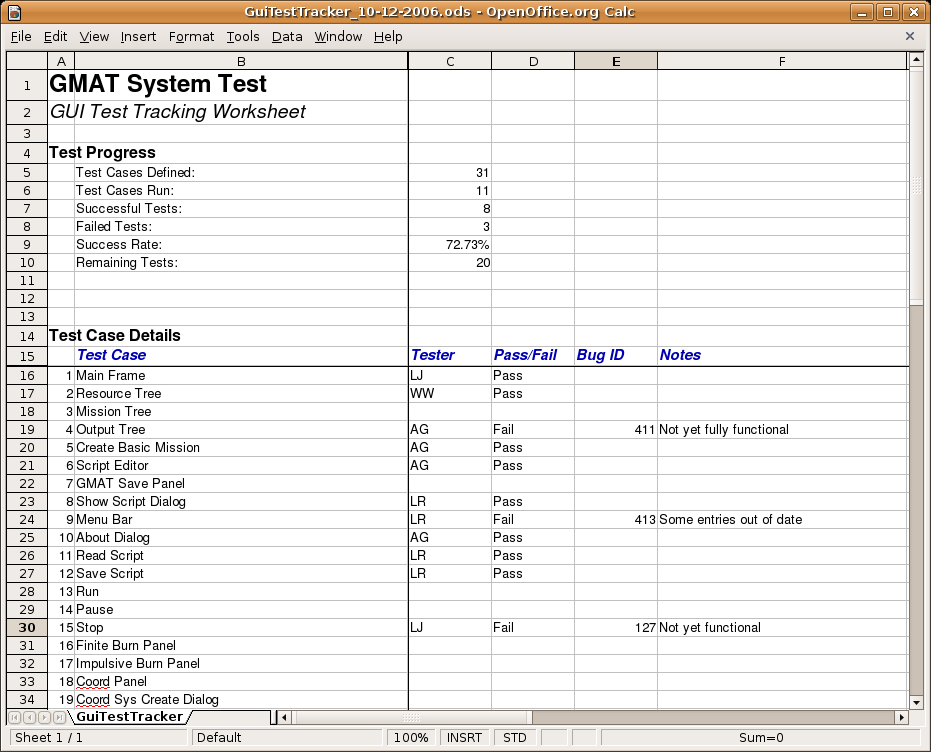
\includegraphics[460,372]{Images/GuiTestTracker.png}
\caption{\label{figure:GuiTestTracker}The GUI Test Tracking Spreadsheet}
\end{center}
\end{figure}

\section{GUI Test Case Management}

The GUI test cases are managed using a test tracking spreadsheet generated at the end of test
preparation, described in Chapter~\ref{chap:testprep}.  Figure~\ref{figure:GuiTestTracker} shows an
example of this spreadsheet partway through a testing cycle.

The test procedure for GUI based tests requires extensive exercising of the components in the GUI.
Testers follow these steps when executing the system tests:

\begin{enumerate}
\item\label{item:GetGuiTestcases} Obtain the latest versions of the GUI test cases and a local copy
of the test case tracking spreadsheet\footnote{The test tracking spreadsheet is generated from the
Systen Test Matrix spreadsheet using an OpenOffice macro, as described in
Section~\ref{section:CompleteCoverage}.}.
\item Identify the tests that the tester needs to run.
\item Open GMAT\footnote{GMAT should only be opened one time for any given testing period.  All
tests run during that test period -- typically a morning or afternoon -- should be run in the same
instance of GMAT.  This helps ensure that the system is stable over long periods of time.  If the
system is shut down, either by the user or through a system crash, that event should be noted.}.
\item Run each test following the procedure in Section~\ref{section:RunningGuiTests}.
\item As each test is run, record the results of the test on the test case worksheet retrieved in
step~\ref{item:GetGuiTestcases}.
\item When anomalies are found in testing, record them on the test case worksheet and enter them in
the bug tracking database.
\item Close GMAT at the end of the test period.
\item At the end of each day or when testing is finished, whichever occurs first, gather the
completed test case worksheets and place them in the folder used to gather the test results.
\item At the end of each day or when testing is finished, whichever occurs first, save the local
gui test tracking spreadsheet with the name <spreadsheetName>\_<tester's initials> in the folder
used to gather the test results.
\item Upon completion of all assigned test cases, report that status to the system test lead.
\end{enumerate}

The procedure for running a single test case is described next.

\section{\label{section:RunningGuiTests}Running the GUI System Tests}

By their very nature, the script based tests described in Chapter~\ref{chap:scripttests} follow a
linear execution sequence once the scripts have been written and debugged.  In contrast,
interactions performed using the GMAT GUI are less structured -- users can use the controls on the
GUI in a seemingly random fashion -- so the test cases for the GUI include allowances for
interacting with the GUI elements by the tester in a more free form manner than the script based
tests allow.

\subsection{Sample GUI Test Case}

A sample GUI test case is shown here:

\begin{quote}
\VerbatimInput[numbers=left,firstnumber=1]{./SystemTests/OpenGLPanel.txt}
\end{quote}

\begin{figure}[htb]
\begin{center}
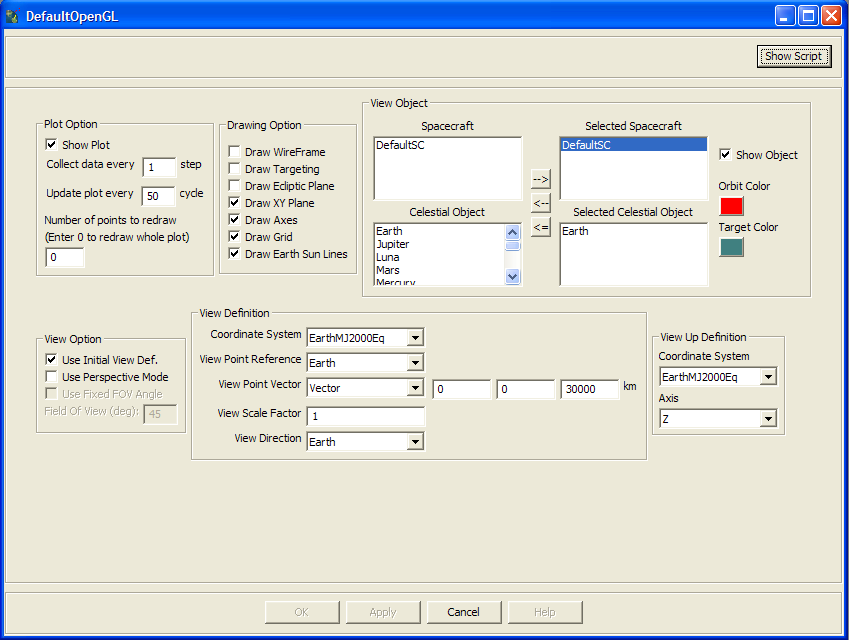
\includegraphics[300,235]{Images/OpenGLPanel.png}
\caption{\label{figure:openGLPanel}The OpenGLPlot Setup Panel}
\end{center}
\end{figure}

\noindent The test case worksheet shown here is the test case for the OpenGL plot setup panel.
The panel, shown in Figure~\ref{figure:openGLPanel}, is a fairly complex GUI panel,
containing text fields, combo boxes, check boxes, text lists, and action buttons which open color
selection dialogs.  Each element is included in the test plan worksheet, along with the standard
control processes that need to be exercised.  Each test criterion is evaluated using this worksheet,
and given a pass or fail evaluation.

\subsection{Procedure}

Each GUI test case has a worksheet like the one shown above.  A tester follows this procedure to
perform the associated system test:

\begin{enumerate}
\item Open the test case worksheet.
\item Follow the procedure outlined in the test case.
\begin{itemize}
\item Section~\ref{section:TestRules} provides detailed instructions about the process that should
be followed when testing each type of GUI element.
\item Each item identified in the worksheet is marked as either passing or failing the test.  If
the item fails, an associated bug is entered or identified in the bug tracking system and listed on
the worksheet.
\item After completing the tests on the worksheet, the tester experiments with the component for an
additional period (typically ten to fifteen minutes), checking to be sure that the component is
stable and behaves correctly when bad data is entered, and when random actions are taken using that
component.
\item Once every item on the worksheet has been evaluated and the final period of usability testing
has been performed, the number of pass and fail evaluations are counted and recorded in the
summary section of the test case worksheet. Any bugs identified on the worksheet are listed in this
section, and any additional notes that need to be recorded are also listed here\footnote{These data
are collected using an automation tool to build a status report for the system tests.}.
\end{itemize}
\item Summarize the results of the tests.
\begin{itemize}
\item Once every item on the worksheet has been evaluated, an overall pass or fail evaluation is
made and recorded in the summary section.  Any bugs identified on the worksheet are listed in this
section, and any additional notes that need to be recorded are also listed here.
\item Add the tester's name and the data the test was run to the worksheet.
\item Save the completed test case worksheet.
\end{itemize}
\item Update the local test tracking worksheet to indicate that the test was run and the results of
the run.
\item Save the test tracking worksheet.
\end{enumerate}

\subsection{Reporting Results}

At the start of the system test process, a central location was established for collection of the
test results.  The final step performed by the system testers is to copy their test case worksheets
and local test tracking worksheet to this central location.  This action is performed each day the
system tests are run so that the progress of the system test execution can be evaluated.  Upon
completion of all system testing by a specific tester, a final update is made and the system test
lead is notified that that tester has completed the assigned tests.  Chapter~\ref{chap:reporting}
describes the consolidation of the collected test results into a system test report.

\section{\label{section:TestRules}Procedural Rules}

The steps described in the preceding sections lay out the procedures followed when testing the GUI
elements of GMAT.  In this section, the criteria that must be evaluated are defined for these
tests.

\subsection{\label{Sec:GeneralTests}Test Procedures for All Elements}


%  This is the list of tests associated with panel aesthetics
\noindent\textbf{Aesthetics}\\

\noindent Description:  This set of tests is to verify look and feel
of a panel.

%
\begin{itemize}
    \item Can all of the data input fields be seen at the default panel
    size for all tabs on panel?  This includes bounding boxes.
    %
    \item Is there too much blank space surrounding the data area?
    %
    \item Is there too little blank space surrounding the data area?
    %
    \item Can the window be resized so that the data cannot be seen?
    %
\end{itemize}
\vspace{.25 in}

%
\noindent\textbf{General Panel Functionality}\\

\noindent Description:  This is the list of tests associated with
basic  panel functionality: open, close, rename, minimize, ok,
cancel, help, show script, command summary.

\begin{itemize}
    %
    \item From the appropriate tree (Resource or Mission), can you create a new object of the type being tested?
    %
    \item Can you double left click and open the panel of the new
    object?
    %
    \item Can you rename the new object?
    %
    \item If there is a default object of the type being tested, can you rename
    it?  Check at least one place in the mission sequence or resource tree to
    ensure the new name is being used.
    %
    \item Can you make a minor change on the panel, hit ok, and then rename the object?
    %
    \item Can you make a minor change on the panel, hit ok, reopen,
    and see that the change was saved?
    %
    \item Can you make a minor change on the panel, hit apply, then
    hit show script to see that the apply button saved the change
    and  it is visible in the script?
    %
    \item Can you open the panel, and while the panel is open,
    change the name in the resource tree.  Check at least one place in the mission sequence or resource tree to
    ensure the new name is being used.
    %
    \item Can you open the panel and hit cancel and the panel
    closes?
    %
    \item Can you open the panel, make a minor change in the data,
    hit cancel, reopen the panel and confirm the data was not saved?
    %
    \item Can you open the panel and
    click the small ``x" button in the upper right hand corner and close the panel?
    %
    \item Can you open the panel, make a minor change in the panel,
    click the small x button in the upper left hand corner, and be
    prompted to save data before closing?
    %
    \item When you click the minimize icon does the panel minimize?
    %
    \item When the panel is minimized, can you hit the maximize icon
     and the panel reopens to previous size?
    %
    \item When the panel is open and you use the tab key to
    negotiate panel, does the action agree with style and GUI
    philosophy?
\end{itemize}
\vspace{.25 in}

%
\noindent\textbf{Panel Data Element Completeness and Correctness}\\

\noindent Description: This set of tests verifies that all data
elements that should appear on the panel indeed appear on the panel.
It also tests that all elements that should appear in show script
appear there and that items that should not appear in show script do
not appear there.

\begin{itemize}
    %
    \item Verify that only data elements that occur in the Range
    Test Plan appear in show script and that the user does not see
    any other object fields.   Also check that defaults agree with
    Range Test Plan.
    %
    \item Verify that all elements that should appear in show script
    appear.  (See range test plan)
    %
    \item  Verify that all data elements
    that appear in Show Script also appear on the GUI.  This
    means that if you can set something in the script, ensure that it
    appears in the GUI.
    %
\end{itemize}
\vspace{.25 in}


\subsection{Procedures for Specific Control Types}
The following table provides additional guidelines that should be followed when testing each
specific type of control.
 \begin{longtable}{p{1.25 in} |p{4.5 in} }
 \caption
 [Tests for Data Objects on All Panels]
 {Tests for Data Objects on All Panels \label{Table:DataElementTests}}\\
 \hline\hline
% \multicolumn{2}{@{*}c@{*}}%
%      {This part appears at the top of the table}\\
 Element Type & Tests\\
 \hline
 \endfirsthead
 \caption[]{(Tests for Data Objects on All Panels...continued)}\\
 \hline\hline
 Element Type & Tests\\
 \hline\hline
 \endhead
 \hline
 % This goes at the&bottom.\\
 \hline
 \endfoot
 \hline
 \hline
 \endlastfoot
%-----------------------------------------------------------------------
%-----------------------Begin Table Here--------------------------------
%-----------------------------------------------------------------------
% ---- Column 1--------%
Check Boxes &
% ---- Column 2--------%
\begin{itemize} \vspace{-.25 in}
\item Set all check boxes to off (unchecked), hit show script, and verify that the functionality is
indeed turned off for each radio button and check box.
%
\item Set all check buttons to on (checked), hit apply, and show script
and verify that the functionality is indeed turned on for each radio
button and check box.
\end{itemize} \\
\hline
% ---- Column 1--------%
Radio Buttons &
% ---- Column 2--------%
\begin{itemize} \vspace{-.25 in}
   \item For each radio button on panel, select the button, and ensure that it activates
   and all others are deactivated.  Hit Apply, and then check show
   script to ensure that the configuration was properly saved.
\end{itemize} \\
\hline
%-------------- This is the beginning of a new row!!!----------------------
% ---- Column 1--------%
Combo Boxes &
% ---- Column 2--------%
\begin{itemize} \vspace{-.25 in}
\item  For each combo box on the panel, ensure that all options that
appear in Range Test Plan appear in the pull down menu.
%
\item  For each Combo box on the panel, select each allowable option, hit apply and show script
and check to see that the option was correctly saved.
%
\item Check to ensure that the combo box is not editable.
\end{itemize} \\
\hline
%-------------- This is the beginning of a new row!!!----------------------
% ---- Column 1--------%
Text Fields &
% ---- Column 2--------%
\begin{itemize} \vspace{-.2 in}
\item For each text field enter ``DNE" and ensure that if GMAT should reject this string that the string is
rejected. ( Currently, this is not an acceptable value for any GMAT
field unless the user has created an appropriate object type and
named it DNE, and is using it correctly in the GUI. )
%
\item Perform all range tests as described in Range Test Plan.
%
\item For all numeric fields, enter an allowed numeric value, hit
apply and show script and check that the value was saved.
%
\item If user-defined objects can appear in the combo box, create
one object for all allowable object types for the particular combo
box, and ensure that it appears in the combo box.  Also, hit apply
and ensure that each case appears in show script.
%
\end{itemize} \\
\hline
%-------------- This is the beginning of a new row!!!----------------------
% ---- Column 1--------%
Action Buttons &
% ---- Column 2--------%
\begin{itemize} \vspace{-.2 in}
\item For each button ensure that clicking on the button brings up the appropriate panel.
\item For the panel opened up, perform all tests defined in Section \ref{Sec:GeneralTests} and Table \ref{Table:DataElementTests}
\end{itemize} \\
\hline
%-------------- This is the beginning of a new row!!!----------------------
% ---- Column 1--------%
Selection Lists &
% ---- Column 2--------%
\begin{itemize} \vspace{-.2 in}
\item First Item
\item Second Item
\end{itemize} \\
\hline

%-------------- This is the beginning of a new row!!!----------------------
% ---- Column 1--------%
Tabbed Panels &  % ---- Column 2--------%
\begin{itemize} \vspace{-.2 in}
\item First Item
\item Second Item
\end{itemize} \\
\end{longtable}


%% ---- Column 2--------%
%\begin{itemize} \vspace{-.2 in}
%\item First Item
%\item Second Item
%\end{itemize} \\
%\hline


\subsection{Usability Testing}

The tests described in the preceding paragraphs are meant to exercise all of the elements of the
graphical user interface.  One important aspect of the interface not covered by those tests is the
usability of the system: the GUI may perform error free as designed, and still be difficult to use
in practice.  Usability testing is performed to capture information about this aspect of the GUI.

